\section{\textit{Range Doppler Map}}

\subsection{Génération des Signaux Radar}

Les signaux radar sont générés selon deux méthodes distinctes : la Figure 4 et l'équation 16 des principes du radar FMCW \footnote{Fig 4 et eq (16) du pdf RadarFMCW du cours}. Chaque méthode est appliquée à chaque \textit{chirp} et le résultat est stocké dans une matrice NxK. Les matrices résultantes, \(NxK^{(\text{Fig.4})}\) et \(NxK^{(\text{Eq.16})}\), représentent les signaux générés pour chaque échantillon de fréquence Doppler \(K\) et chaque instant de temps \(N\). 

\subsection {Obtention de la RDM}

La RDM est obtenue grâce à plusieurs transformée de Fourier. La première transformée se fait sur chaque colonne de la matrice NxK. La deuxième se fait sur les lignes de la matrice obtenu après la première transformée. La dernière est une transformée de Fourrier 2D. L'étape finale consiste à sommer les RDM obtenues pour chaque cibles pour n'en avoir qu'une seule au final. La figure \ref{fig:RDM_2_ways} montre les RDM obtenues selon les deux méthodes. Elle permet aussi de montrer qu'il n'y a pas de différences entre l'utilisation de l'équation 16 ou de la figure 4. 

\begin{figure}[H]
  \centering
  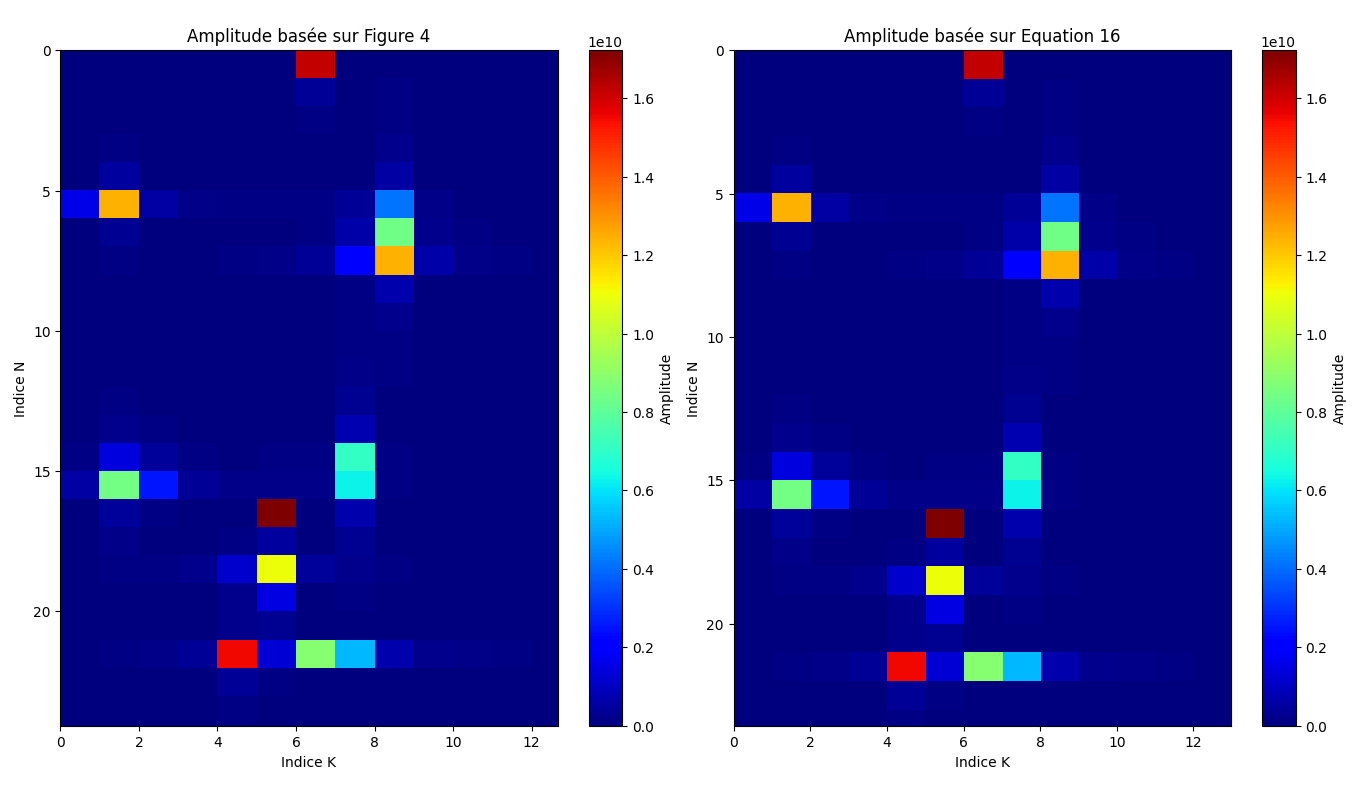
\includegraphics[scale =0.4]{Pictures/RDM_P_SST.png}
    \caption{RDM obtenues par deux moyens différents}
    \label{fig:RDM_2_ways}
\end{figure}

Sur base de la figure \ref{fig:RDM_2_ways} et des définitions des résolutions ( $\Delta R_0 = \frac{c}{2B} = 0,75 m$ et $\Delta v = \frac{c}{2KTF_c} = 0.24 m/s$), il est possible de retrouver approximativement les positions et vitesses des différentes cibles en multipliant les indices K et N par leurs résolutions. Le tableau \ref{tab:results_calc_RDM} montre les résultats ainsi calculés. Il est important de noter que seul des vitesses et des distances positives ont été prises en compte dans le cadre de ce projet.  

\begin{table}[H]
    \centering
    \begin{tabular}{|c|c|c|c|c|c|}
    \hline
    \rowcolor[gray]{0.90} $R_0$ [m] &  $v$ [m/s] &  $N$ [ ] &  $K$ [ ] & $R_{0_{estimé}}$ [m] &  $v_{estimé}$ [m/s]  \\\hline
 5,41  & 1,88 & 7  & 8 & 5,25  & 1,92 \\\hline
 11,11 & 0,33 & 15 & 1 & 11,25 & 0,24 \\\hline
 12,10 & 1,23 & 16 & 5 & 13,50 & 1,20 \\\hline
 15,96 & 1,01 & 21 & 4 & 15,75 & 0,96 \\\hline
 4,22  & 1,90 & 6  & 8 & 4,50  & 1,92 \\\hline
 13,80 & 1,16 & 18 & 5 & 13.50 & 1,20 \\\hline
 10,94 & 1,68 & 14 & 7 & 10,50 & 1,68 \\\hline
 3,65  & 0,18 & 5  & 1 & 3,75  & 0,24 \\\hline
 0,10  & 1,47 & 0  & 6 & 0,00  & 1,44 \\\hline
 15,89 & 1,57 & 21 & 6 & 15,75 & 1,44 \\\hline
    \end{tabular}
    \caption{vitesses réelles, vitesses mesurées et indices sur la RDM}
    \label{tab:results_calc_RDM}
\end{table}

\subsection{Discussion sur le Choix des Paramètres}

Afin de discuter de la pertinence des paramètres choisis étant donné la situation qui est analysée, il faut calculer la portée maximale estimée $\left(\frac{cTF_s}{2B}\right)$  ainsi que l'intervalle d'estimation de la vitesse $\left(\frac{c}{4TF_c}\right)$. Ces deux valeurs valent respectivement 150 m et 31,25 m/s avec les paramètres choisis. En sachant que la distance maximale est de 20 m et que la vitesse maximale est de 2 m/s, il n'y a que 13,3\% de la portée maximale qui est exploitée et seulement 6,4\% de l'intervalle de vitesse qui est exploité. Ceci ainsi que le calul des résolutions fait au point précédent montre que les paramètres du radar ne sont pas choisis de manière optimal pour l'application visée. En augmentant $B$ et $F_c$, il serait possible d'avoir de meilleurs résolutions ainsi qu'une meilleur utilisation de la RDM. 
